%\documentclass[handout]{ximera}
\documentclass{ximera}

\usepackage{gensymb}
\usepackage{tabularx}
\usepackage{mdframed}
\usepackage{pdfpages}
%\usepackage{chngcntr}

\let\problem\relax
\let\endproblem\relax

\newcommand{\property}[2]{#1#2}




\newtheoremstyle{SlantTheorem}{\topsep}{\fill}%%% space between body and thm
 {\slshape}                      %%% Thm body font
 {}                              %%% Indent amount (empty = no indent)
 {\bfseries\sffamily}            %%% Thm head font
 {}                              %%% Punctuation after thm head
 {3ex}                           %%% Space after thm head
 {\thmname{#1}\thmnumber{ #2}\thmnote{ \bfseries(#3)}} %%% Thm head spec
\theoremstyle{SlantTheorem}
\newtheorem{problem}{Problem}[]

%\counterwithin*{problem}{section}



%%%%%%%%%%%%%%%%%%%%%%%%%%%%Jenny's code%%%%%%%%%%%%%%%%%%%%

%%% Solution environment
%\newenvironment{solution}{
%\ifhandout\setbox0\vbox\bgroup\else
%\begin{trivlist}\item[\hskip \labelsep\small\itshape\bfseries Solution\hspace{2ex}]
%\par\noindent\upshape\small
%\fi}
%{\ifhandout\egroup\else
%\end{trivlist}
%\fi}
%
%
%%% instructorIntro environment
%\ifhandout
%\newenvironment{instructorIntro}[1][false]%
%{%
%\def\givenatend{\boolean{#1}}\ifthenelse{\boolean{#1}}{\begin{trivlist}\item}{\setbox0\vbox\bgroup}{}
%}
%{%
%\ifthenelse{\givenatend}{\end{trivlist}}{\egroup}{}
%}
%\else
%\newenvironment{instructorIntro}[1][false]%
%{%
%  \ifthenelse{\boolean{#1}}{\begin{trivlist}\item[\hskip \labelsep\bfseries Instructor Notes:\hspace{2ex}]}
%{\begin{trivlist}\item[\hskip \labelsep\bfseries Instructor Notes:\hspace{2ex}]}
%{}
%}
%% %% line at the bottom} 
%{\end{trivlist}\par\addvspace{.5ex}\nobreak\noindent\hung} 
%\fi
%
%


\let\instructorNotes\relax
\let\endinstructorNotes\relax
%%% instructorNotes environment
\ifhandout
\newenvironment{instructorNotes}[1][false]%
{%
\def\givenatend{\boolean{#1}}\ifthenelse{\boolean{#1}}{\begin{trivlist}\item}{\setbox0\vbox\bgroup}{}
}
{%
\ifthenelse{\givenatend}{\end{trivlist}}{\egroup}{}
}
\else
\newenvironment{instructorNotes}[1][false]%
{%
  \ifthenelse{\boolean{#1}}{\begin{trivlist}\item[\hskip \labelsep\bfseries {\Large Instructor Notes: \\} \hspace{\textwidth} ]}
{\begin{trivlist}\item[\hskip \labelsep\bfseries {\Large Instructor Notes: \\} \hspace{\textwidth} ]}
{}
}
{\end{trivlist}}
\fi


%% Suggested Timing
\newcommand{\timing}[1]{{\bf Suggested Timing: \hspace{2ex}} #1}




\hypersetup{
    colorlinks=true,       % false: boxed links; true: colored links
    linkcolor=blue,          % color of internal links (change box color with linkbordercolor)
    citecolor=green,        % color of links to bibliography
    filecolor=magenta,      % color of file links
    urlcolor=cyan           % color of external links
}

\title{Symmetries}
\author{Bart Snapp and Brad Findell}

\outcome{Learning outcome goes here.}

\begin{document}
\begin{abstract}
Abstract goes here.  
\end{abstract}
\maketitle

\begin{teachingnote}
\end{teachingnote}

\begin{definition}
A symmetry is a transformation that takes a figure onto itself.  
\end{definition}
\begin{problem}
List the symmetries of an equilateral triangle.  Explain how you know you have them all.  
\end{problem}

\begin{problem}
Flip through these notes and describe the symmetries you notice.  Try to find reflection symmetry, rotation symmetry, and translation symmetry.  
\end{problem}

\begin{teachingnote}
To augment the examples, bring some pictures from Web.   Tesselations and Frieze patterns are necessary for translation symmetry.  
\end{teachingnote}

\begin{problem}
Suppose the symmetries of a square are called $R_0$, $R_{90}$, $R_{180}$, $R_{270}$, $V$, $H$, $D$, $D'$, based upon the figure below.  
\begin{image}
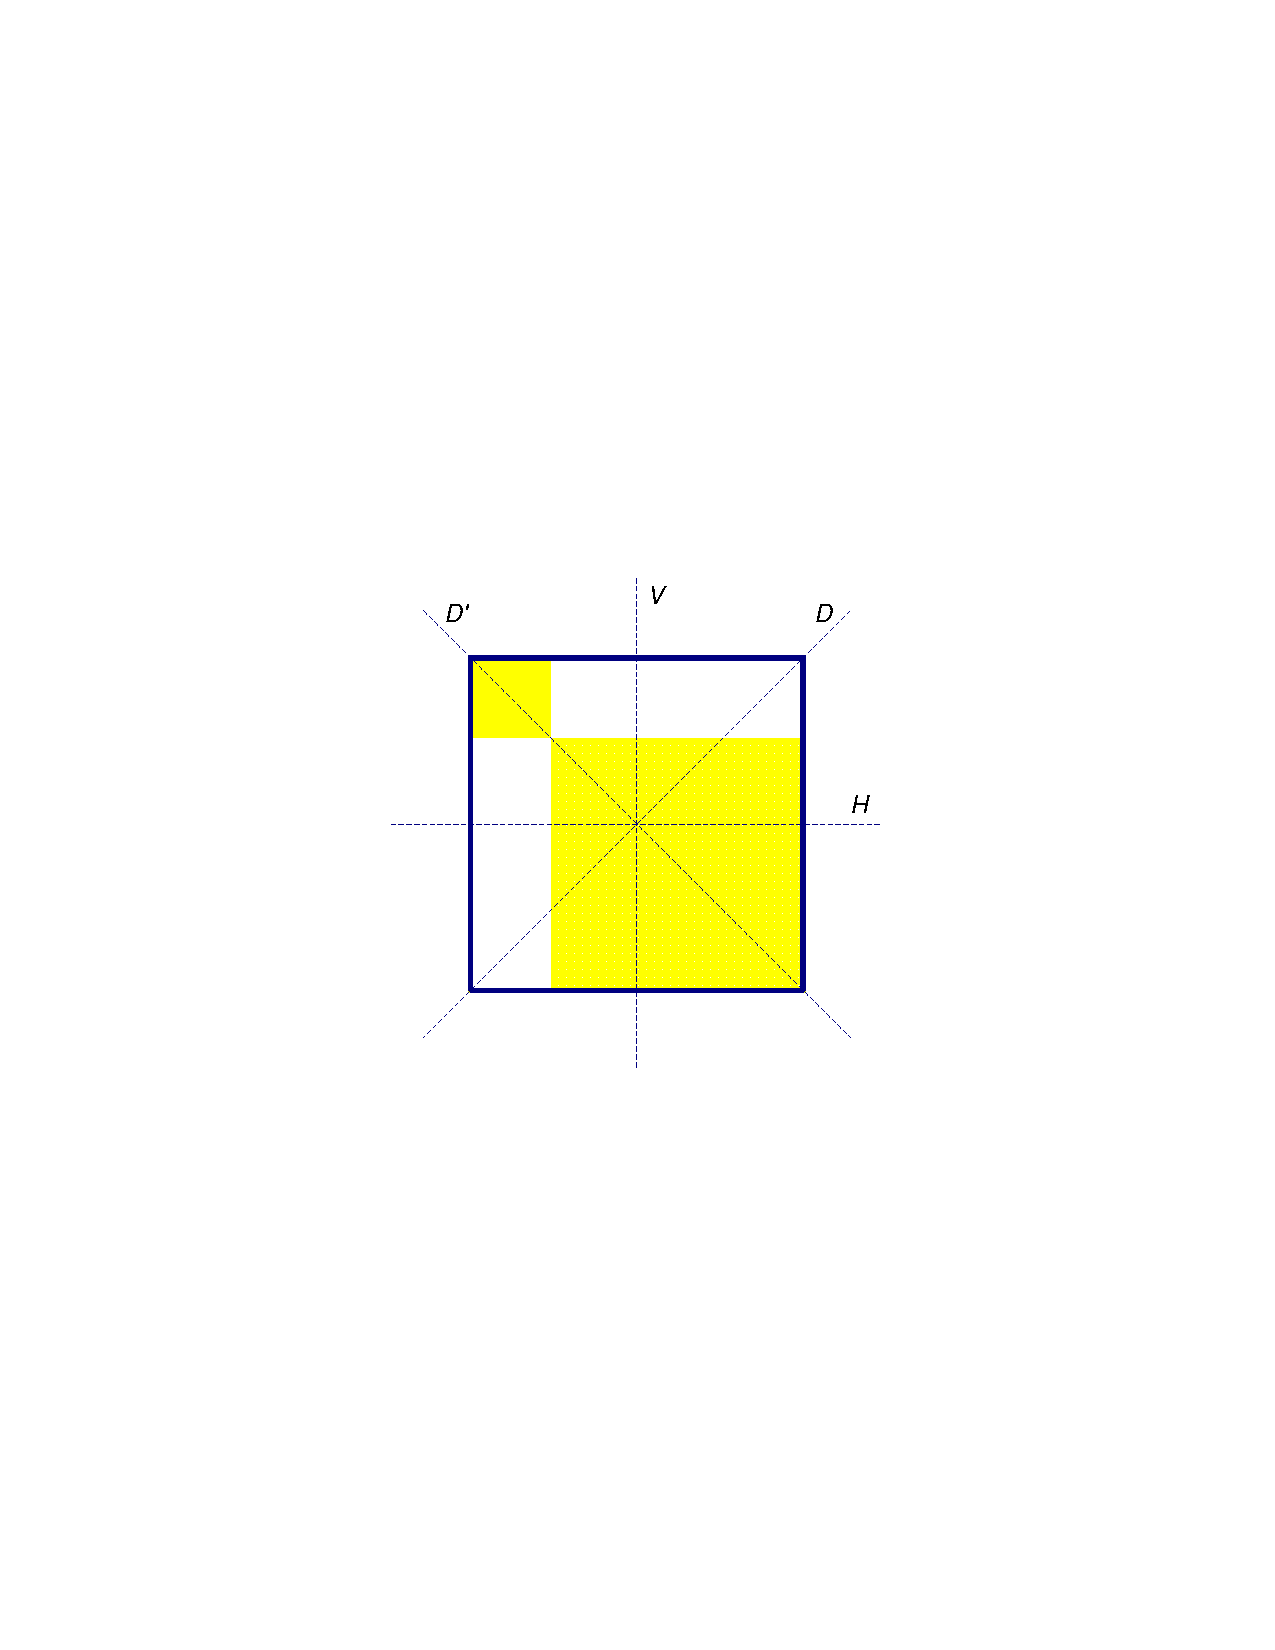
\includegraphics[scale=0.6]{D4.pdf}
\end{image}
Hint:  To identify a single transformation that accomplishes a sequence of transformations, do the transformations physically with a square piece of paper marked with ``FRONT'' on the side that starts facing you.  Or mark the corners of the square with $A$, $B$, $C$, and $D$.  
\begin{enumerate}
\item Complete the following table, where the entry at (row, column) is the symmetry that results from the sequence of symmetries given by the row heading followed by the column heading.  
\item What patterns and not-quite-patterns do you notice in the table?  For example, which elements ``commute'' with which other elements?
\item What facts about isometries can you observe in the table?  For example, what can you say generally about sequences of rotations and reflections?  
\end{enumerate}
\[
{\arraycolsep=12pt\def\arraystretch{3}
\begin{array}{|l||l|l|l|l||l|l|l|l|}
\hline
 & R_0 & R_{90} & R_{180} & R_{270} & V & H & D & D' \\ \hline\hline
R_0 & & & & & & & & \\ \hline
R_{90} & & & & & & & & \\ \hline
R_{180} & & & & & & & & \\ \hline
R_{270} & & & & & & & & \\ \hline\hline
V & & & & & & & & \\ \hline
H & & & & & & & & \\ \hline
D & & & & & & & & \\ \hline
D' & & & & & & & & \\ \hline
\end{array}
}\]
\end{problem}

\begin{teachingnote}
Blurring one's eyes, it is possible to notice (1) the composition of a reflection and a rotation (in either order) is a reflection; (2) the composition of two rotations is a rotation; and (3) the composition of two reflections is a rotation.  Looking a bit closer, one can see that some elements commute with one another and others do not.  
\end{teachingnote}
\end{document}
